\documentclass{article}

\usepackage{natbib}
\usepackage{graphics}
\usepackage{amsmath}
\usepackage{indentfirst}
\usepackage[utf8]{inputenc}

% \VignetteIndexEntry{massiR_Example}

\usepackage{Sweave}
\begin{document}
\Sconcordance{concordance:massiR_vignette.tex:massiR_vignette.Rnw:%
1 10 1 1 0 16 1 1 2 1 0 1 1 3 0 1 2 2 1 1 2 4 0 1 2 6 1 1 2 4 0 2 2 4 0 %
1 2 2 1 1 4 2 1 1 14 1 2 9 1 1 2 4 0 2 2 8 0 1 2 7 1 1 3 5 0 1 2 7 1 1 %
2 4 0 1 2 1 1 1 2 4 0 2 2 13 0 1 2 6 1 1 2 4 0 1 2 4 1 1 4 1 2 6 1 1 19 %
1 2 6 1 1 5 1 2 37 1}


\title{massiR: MicroArray Sample Sex Identifier}
\author{Sam Buckberry}
\maketitle

\section{The Problem}
Given that the sex of many species is an easily observable and usually unambiguous classification, it is surprising the number of microarray datasets in public repositories that lack the associated sample sex information. Sex-biased gene expression in normal and pathological tissues is a well recognised for both sex chromosome and autosomal genes. Sex biases also exist in the prevalence and severity of many common human diseases, such as cardiovascular disease and some cancers. As sex is a potential influencing factor of both pathological and non-pathological phenotypes, gene expression analyses that do not account for sex-specific effects could fail to identify a significant proportion of genes that contribute the condition under investigation. Therefore, the absence of sample sex information restricts the reuse of gene expression datasets where the researcher intends to factor the effect of sex in reanalysis or reinterpretation, or when intending to include such datasets in larger gene expression meta-analyses. 

This is why we developed MASSI, an R package for predicting the sex of samples in microarray datasets. The massi package allows researchers to expand their analyses to retrospectively incorporate sex as a variable, generate or confirm sex information associated with publicly available datasets, or to accurately predict the sex of samples missing sex information.
\clearpage

\section{Importing data to use in the massiR analysis}
The massi analysis begins by importing a standard gene expression data of normalised and log transformed probe values. The gene expression data can be in the form of a data.frame object and have the sample identifiers as the column names and the probe identifiers as the row names, or as an ExpressionSet object. The Y chromosome probe identifiers must be as a data.frame object with the probe identifiers as row.names.   

To load the included test massi gene expression matrix:
\begin{Schunk}
\begin{Sinput}
> library(massiR)
> data(massi.test.dataset)
\end{Sinput}
\end{Schunk}
The included gene expression matrix is composed of 60 samples and 1026 probes as a data.frame object.

To load the test probe list corresponding to the included data:
\begin{Schunk}
\begin{Sinput}
> data(massi.test.probes)
\end{Sinput}
\end{Schunk}
The Included list of Y chromosome probes contains 56 probe identifiers as row.names as a data.frame object.

\section{Extracting the Y chromosome probe data}
The first step of the massiR analysis involves extracting the expression values for probes that correspond to Y chromosome genes. When the expression values for Y chromosome probes are extracted, the expression variance for each probe across all samples is calculated. This allows the identification of low variance probes, which are unlikely to be informative in sex classification. The user has the option of selecting a probe variation threshold, so only the most informative probes are used in the classification process. Deciding on a probe variation threshold can be informed by inspecting the automatically generated probe variation plot (Figure 1). In our experience, using the most variable 25-50\% of probes (typically 10-40 probes, depending on platform) produces good results. 

To extract data corresponsing to Y chromosome probes from the test dataset and look at a probe variation plot:

\begin{Schunk}
\begin{Sinput}
> massi.y.out <- massi.y(massi.test.dataset, massi.test.probes)
\end{Sinput}
\end{Schunk}

\begin{Schunk}
\begin{Sinput}
> massi.y.plot(massi.y.out)
\end{Sinput}
\end{Schunk}

The plot pictured below is output to the R graphics device.

\setkeys{Gin}{width=1\linewidth}
\begin{figure}
\begin{center}
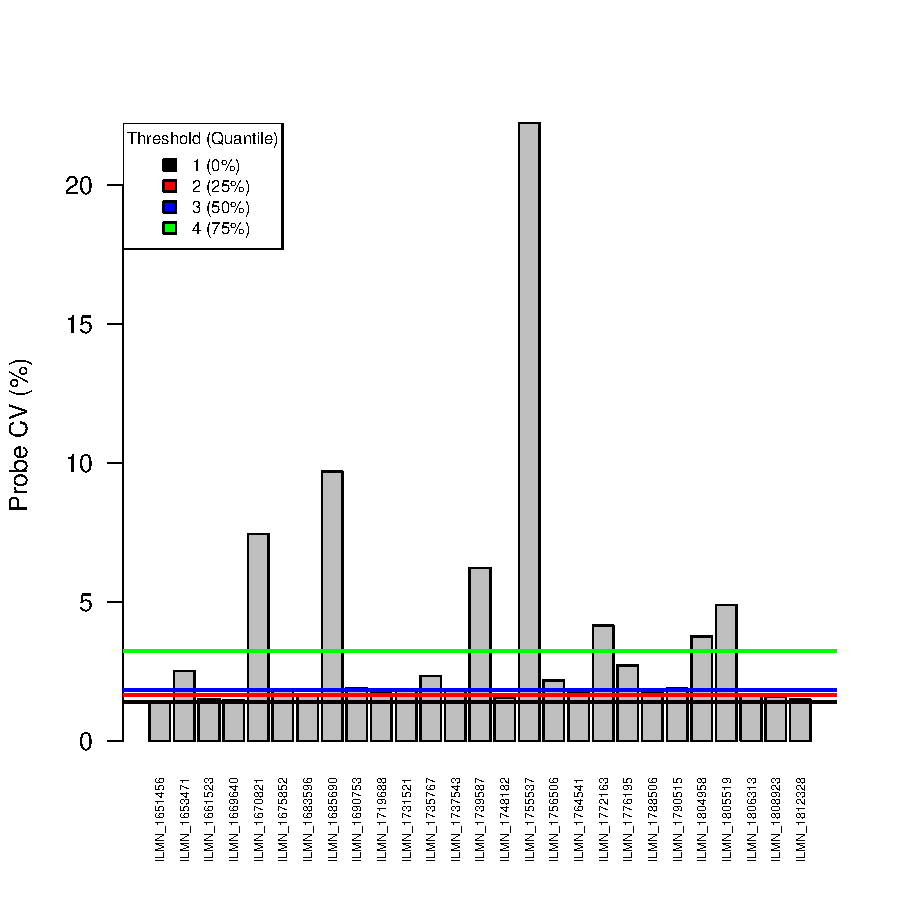
\includegraphics{massiR_vignette-fig1}
\end{center}
\caption{Expression variation (CV) of Y chromosome probes across all samples}
\label{fig:fig1}
\end{figure}

\clearpage

You have the option of using you own list of probes corresponding to Y chromosome genes or using the probe lists included with the package. The included lists correspond to popular microarray platforms and contain identifiers for probes that map uniquely to Y chromosome genes.

To load all the included probe lists:
\begin{Schunk}
\begin{Sinput}
>  data(y.probes)
\end{Sinput}
\end{Schunk}
Check the names of the platforms for the probe lists.
\begin{Schunk}
\begin{Sinput}
>   names(y.probes)
\end{Sinput}
\begin{Soutput}
[1] "illumina_humanwg_6_v1" "illumina_humanwg_6_v2" "illumina_humanwg_6_v1"
[4] "illumina_humanht_12"   "affy_hugene_1_0_st_v1" "affy_hg_u133_plus_2"  
\end{Soutput}
\end{Schunk}
The names of the probe lists correspond to Ensembl biomart attribute names.

After viewing the probe variation plot, a decision can be made regarding which probes to use in the clustering step. The massiR package includes methods for selecting probe variation thresholds based on quantiles. The threshold can be determined by quantiles of probe variance (CV): 1=All probes, 2=Upper 75\%, 3=Upper 50\%, 4=Upper 25\%. It is highly recommended that probe CV plot generated using the massi.y.plot function be inspected to inform threshold choice (Figure 1). The default threshold value is 3.



Once a probe threshold has been decided upon, run the massi.select function. This will return a data.frame with the samples as columns and the subset of selected y chromosome probes as row names.

\begin{Schunk}
\begin{Sinput}
> massi.select.out <- 
+   massi.select(massi.test.dataset, massi.test.probes, threshold=4)
\end{Sinput}
\end{Schunk}

For instructions on obtaining probe identifiers for other platforms, see the section "Using biomaRt to obtain y chromosome probe lists"

\section{Predicting the sex of samples}

To classify samples as either male or female, clustering is performed using the values from the subset of Y chromosome probes  by implementing the partitioning around medoids algorithm to perform k-medoids clustering (Hennig 2013), where samples are assigned to one of two clusters. The two clusters are then compared using the probe expression values across all samples in each cluster. Samples within the cluster featuring the highest Y chromosome probe values are classed as male and those amongst the cluster with the lowest Y probe values classed as female. Results such sample probe mean, standard deviation and z-scores are reported in a table together with the sex predicted for each sample.

To predict the sex of the samples:
\begin{Schunk}
\begin{Sinput}
> results <- massi.cluster(massi.select.out)
\end{Sinput}
\end{Schunk}

Extract the results for each sample:
\begin{Schunk}
\begin{Sinput}
> sample.results <- data.frame(results[[2]])
\end{Sinput}
\end{Schunk}

\begin{Schunk}
\begin{Sinput}
> head(sample.results)
\end{Sinput}
\begin{Soutput}
  sample_ID mean_y_probes_value y_probes_sd sample_z_score sample_sex
1       S10            6.749520   0.8418586      0.7635561       male
2       S11            5.689586   0.4750484     -1.1143145     female
3       S12            6.702993   0.7894613      0.6920061       male
4       S13            5.838450   0.6759924     -0.7272448     female
5       S14            5.819845   0.6593184     -0.7607977     female
6       S15            5.873285   0.8299253     -0.5544343     female
\end{Soutput}
\end{Schunk}

As you can see, it is a relatively straighforward proceedure to produce a table with the predicted sex of each sample.

\section{Visualising the results}

The results of the massi analysis can easily be visualied using the massi.cluster.plot function and the data values derived from the previous steps. 
To run the massi.plot function:
\begin{Schunk}
\begin{Sinput}
> massi.cluster.plot(massi.select.out, results)
\end{Sinput}
\end{Schunk}
This will produce a bar plot of mean values from the subset of Y chromosome probes used in K-medoids clustering (Figure 2), with the bar colours representing clusters with female as red and male as green. This wil also generate a heatmap with dendrogram of Y chromosome probes as rows and individual samples in columns (Figure 3) and a principal component plot showing clusters (Figure 4). 
\clearpage

\begin{figure}
\begin{center}
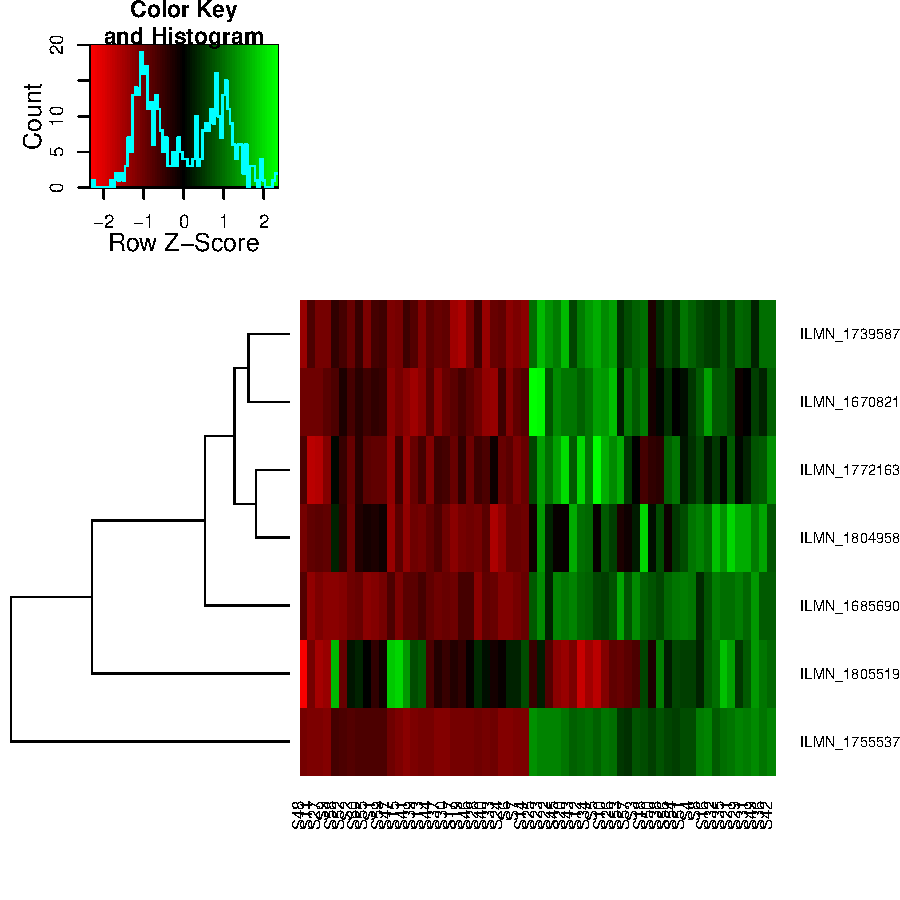
\includegraphics{massiR_vignette-fig2}
\end{center}
\caption{Heat map with dendrogram of Y chromosome probes as rows and individual samples in columns}
\label{fig:fig2}
\end{figure}

\begin{figure}
\begin{center}
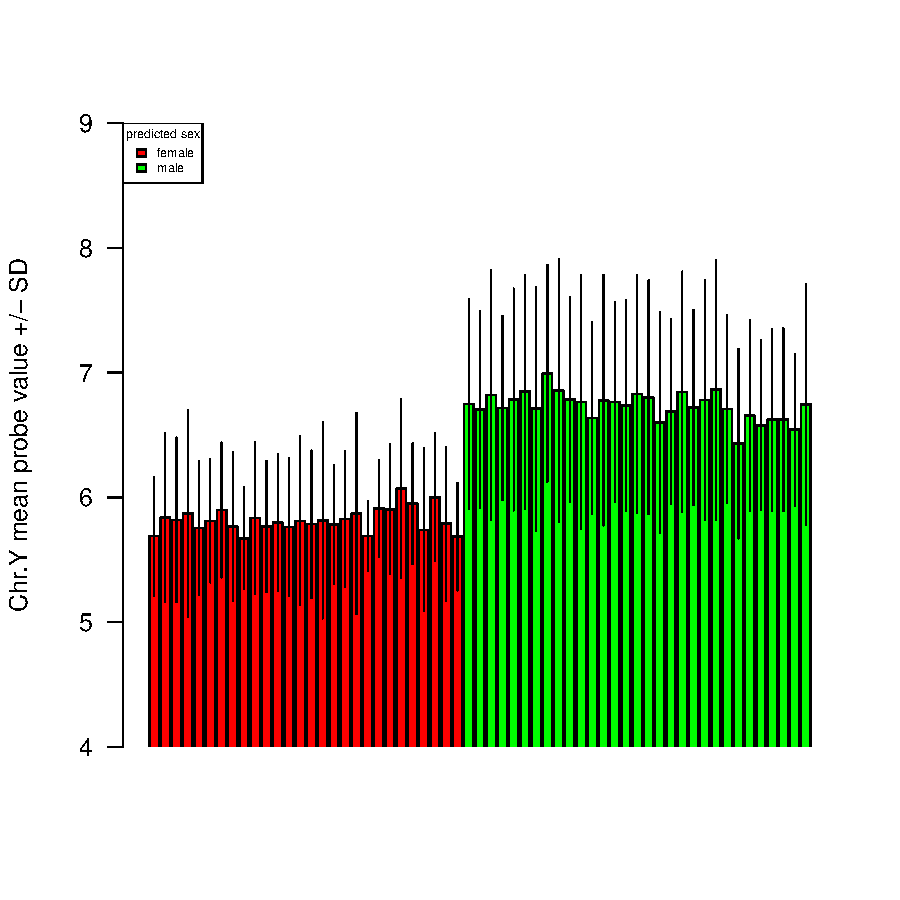
\includegraphics{massiR_vignette-fig3}
\end{center}
\caption{Mean values of the subset of Y chromosome probes used in K-medoids clustering. The bar colours represent clusters, which were assigned as female (red) and male (green)}
\label{fig:fig3}
\end{figure}

\begin{figure}
\begin{center}
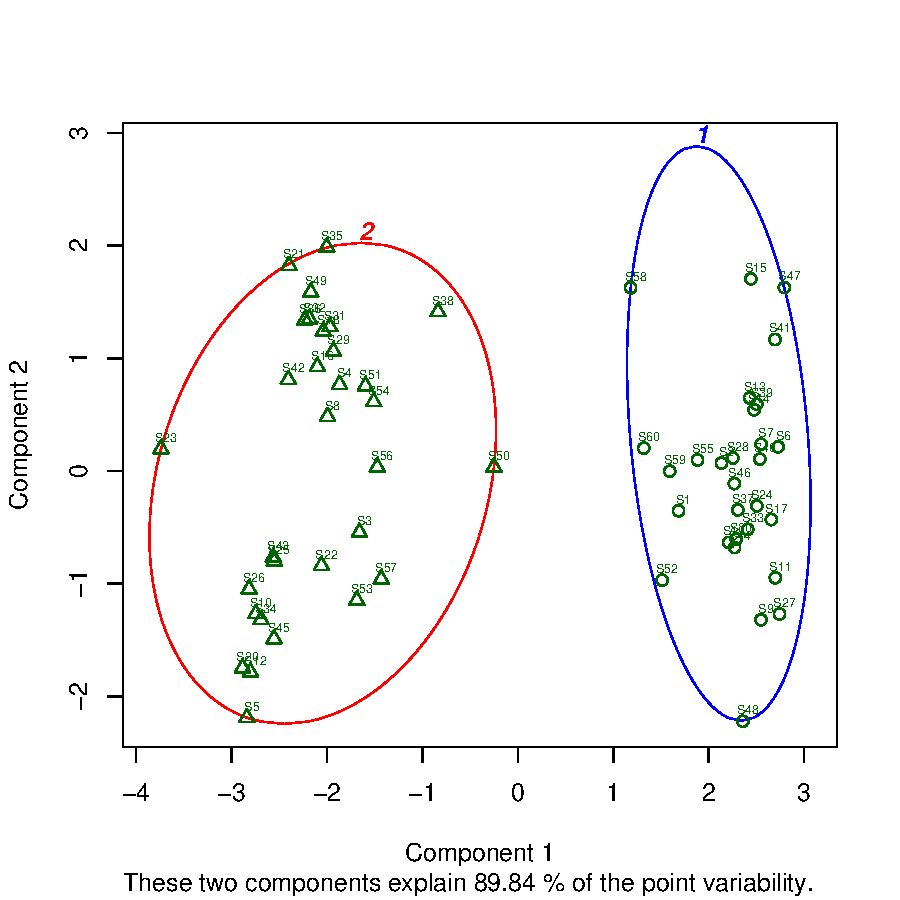
\includegraphics{massiR_vignette-fig4}
\end{center}
\caption{Principal component plot of male and female clusters}
\label{fig:fig4}
\end{figure}

\clearpage

\section{Check for potential sex bias using the dip test}

\section{Using biomaRt to obtain y chromosome probe lists}

\clearpage

\section{References}
  Christian Hennig (2013). fpc: Flexible procedures for clustering.
  R package version 2.1-6.
  http://CRAN.R-project.org/package=fpc
  
  Martin Maechler (2013). diptest: Hartigan's dip test statistic for unimodality - 
  corrected code.
  R package version 0.75-5. http://CRAN.R-project.org/package=diptest
  
  Gregory R. Warnes, Ben Bolker, Lodewijk Bonebakker, Robert Gentleman,
  Wolfgang Huber Andy Liaw, Thomas Lumley, Martin Maechler, Arni Magnusson,
  Steffen Moeller, Marc Schwartz and Bill Venables (2013).
  gplots: Various R programming tools for plotting data.
  R package version 2.12.1.
  http://CRAN.R-project.org/package=gplots
  
  Mapping identifiers for the integration of genomic datasets with the R/Bioconductor package biomaRt.
  Steffen Durinck, Paul T. Spellman, Ewan Birney and Wolfgang Huber, Nature Protocols 4, 1184-1191
  (2009).

  BioMart and Bioconductor: a powerful link between biological databases and microarray data analysis.
  Steffen Durinck, Yves Moreau, Arek Kasprzyk, Sean Davis, Bart De Moor, Alvis Brazma and Wolfgang
  Huber, Bioinformatics 21, 3439-3440 (2005).
  
\end{document}
